This chapter is a basic introduction into the hardware and software tools used for the development of the Single Chip Mote digital system. While the details on the design of this system are presented in later chapters, the purpose of this chapter is simply to introduce these tools and provide basic instructions in their installation and use. This guide is by no means comprehensive and further experimentation and study is required in order to truly understand and master the use of these tools.

\section{Git Repository}
All of the source code and project files for this design is found on the following git repository:
\\ \url{https://repo.eecs.berkeley.edu/git/projects/pistergroup/scm-digital.git}

The repository contains two main directories, one for source code and one for project files specific to the hardware and software development environments. The source code section further divides into hardware and software code, and each of those sections divide further based on FPGA target or software project. The project files directory is also divided into sections for hardware and software IDEs, and each of those sections also divide further based on FPGA target or software project. This hierarchy is shown in Figure \ref{verb:repo-structure}.

\begin{figure}
\begin{verbatim}
/scm-digital
  /proj
    /ise
      /artix7
        /SingleChipMote           # ISE project files for main digital
                                  # system implemented on Artix-7
        /testbench                # ISE project files for testbenches
      /spartan6
        /bootloader               # ISE project files for the bootloading
                                  # hardware implemented on Spartan-6
        /testbenches              # ISE project files for testbenches
        /uRobotDigitalController  # ISE project files for main digital
                                  # system imlpemented on Spartan-6
    /keil
      /firmware                   # Keil project files for bootloading
                                  # software
      /uRobotDigitalController    # Keil project files for main digital
                                  # system software
  /src
    /hw
      /artix7
        /uRobotDigitalController  # Verilog files for main digital system
                                  # implemented on Artix-7
      /spartan6
        /bootloader               # Verilog files for bootloading hardware
                                  # implemented on Spartan-6
        /uRobotDigitalController  # Verilog files for main digital system
                                  # implemented on Spartan-6
    /sw
      /firmware                   # C source and assembly source files
                                  # for bootloading software
      /uRobotDigitalController    # C source and assembly source files
                                  # for main digital system software
\end{verbatim}
\caption{Git repository directory structure}
\label{verb:repo-structure}
\end{figure}


There is also a deprecated repository containing the history of the project during its early development. This repository has been maintained solely for historical purposes:
\\
\url{https://repo.eecs.berkeley.edu/git/projects/pistergroup/singlechip-digital.git}

The information in this user guide is meant for those using the latest source code found on the current repository and may not be applicable to the code found on the deprecated repository.

\section{ARM Cortex-M0 DesignStart Processor} \label{arm-ds}
The digital microprocessor used for this system is the ARM Cortex-M0 DesignStart processor \cite{arm-cm0ds} \cite{cm0ds-architecture}, provided at no cost by ARM for educational purposes. The processor is fully software-compatible with the commercial Cortex-M0; however, the provided Verilog is obfuscated and does not support JTAG debugging.

\section{FPGA Boards}
\subsection{Digilent Nexys 3}
The Digilent Nexys 3 \cite{nexys3-store} is a digital circuit development platform containing the Xilinx Spartan-6 XC6LX16-CS324 FPGA along with various peripherals. The digital system of the Single Chip Mote was originally designed and developed on the Nexys 3 FPGA. This board was chosen because it was the recommended prototyping board to be used with the ARM Cortex-M0 DesignStart processor package. The DesignStart package also came with example projects and Verilog code specifically designed for the Nexys 3 board. However, as the size of the digital system grew, the FPGA on the Nexys 3 could not support the amount of RAM and logic devices needed, and thus the project was moved to the Nexys 4 DDR board. The Nexys 3 is still used for bootloading purposes (see chapter \ref{bootloading} for more information). This board and FPGA is compatible with Xilinx's ISE Design Suite and can also be programmed separately through Digilent's Adept software. % the use of could is justified here

\subsection{Digilent Nexys 4 DDR}
The Digilent Nexys 4 DDR \cite{nexys4-store} is a digital circuit development platform containing the Xilinx Artix-7 XC7A100T-1CSG324C FPGA along with various peripherals. This board is currently used for design, development, and testing of the Single Chip Mote digital system. This board and FPGA is compatible with Xilinx's ISE Design Suite and Vivado Design Suite.


\section{Hardware Development Tools}
\subsection{Xilinx ISE Design Suite 14.6}

\subsubsection{Overview}
Xilinx ISE 14.6 is the integrated development environment used for the hardware development of the Single Chip Mote on both the Artix-7 and Spartan-6 FPGAs. This version of ISE can be download directly from Xilinx, and is known to work on Windows 7 computers. It can also be installed in Windows 8 and 10 with a few extra steps in the installation procedure. This version can also be installed on Linux. Xilinx ISE 14.7 should also work for the purposes of this project; however, this has not been tested or confirmed. % the word should is justified

ISE contains multiple tools required for this project:
\begin{description}
	\item[Project Navigator] The main IDE used to write and synthesize RTL for the FPGA.
	\item[ChipScope Pro] A tool used to create and embed a logic analyzer into an FPGA design for debugging.
	\item[CORE Generator] A tool used to generate Xilinx IP for FPGA designs such as memories, FIFOs, and clock generators.
	\item[ISim] A Verilog simulator.
	\item[iMPACT] A took used to load configuration bitstreams onto FPGAs.
\end{description}

Xilinx has chosen to deprecate its ISE Design Suite in favor of its Vivado Design Suite. However, Vivado supports only 7-series FPGAs, and is not compatible with the Spartan-6 FPGA. Therefore, this project continues to use ISE.

\subsubsection{Installation}
First, download ISE 14.6 from Xilinx \cite{ise-download}. Then, install using the default settings. Once finished the installer may open the license manager and ask for a license. Students and researchers at UC Berkeley may use the license provided to the EECS department for instructional purposes by setting the XILINXD\_LICENSE\_FILE and LM\_LICENSE\_FILE values to 2100@license-srv.eecs.berkeley.edu, as shown in Figure \ref{fig:license-manager}. This license supports all versions of Xilinx tools released prior to October 2015. Xilinx also provides free WEBPACK licenses. % the use of may is justified here

\begin{figure}
\centering
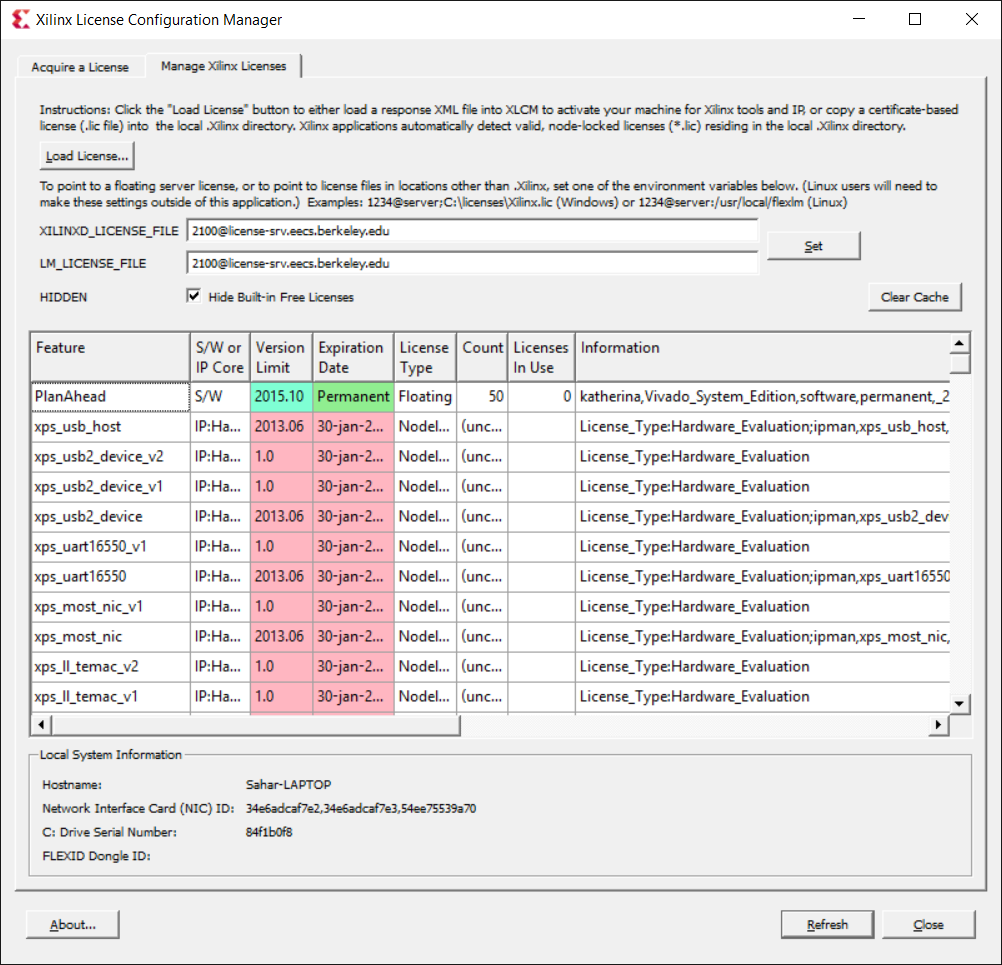
\includegraphics[width=0.7\linewidth]{license-manager}
\caption{Xilinx license manager settings for UC Berkeley license}
\label{fig:license-manager}
\end{figure}

\subsubsection{Additional Install Directions for Windows 8/8.1/10}
Xilinx has also chosen to stop updating and supporting ISE installations, including compatibility updates for Windows 8/8.1/10. ISE 14.6 can still be installed on Windows 8/8.1/10 computers; however, it requires the following modifications \cite{ise-64bit} in order to work:

\begin{enumerate}
	\item Open the following directory: \path{C:\Xilinx\14.6\ISE_DS\ISE\lib\nt64}
	\item Find and rename \path{libPortability.dll} to \path{libPortability.dll.orig}
	\item Make a copy of \path{libPortabilityNOSH.dll} (copy and paste it to the same directory) and rename it \path{libPortability.dll}
	\item Copy \path{libPortabilityNOSH.dll} again, but this time navigate to \path{C:\Xilinx\14.6\ISE_DS\common\lib\nt64} and paste it there
	\item In \path{C:\Xilinx\14.7\ISE_DS\common\lib\nt64} Find and rename\\ \path{libPortability.dll} to \path{libPortability.dll.orig}
	\item Rename \path{libPortabilityNOSH.dll} to \path{libPortability.dll}
\end{enumerate}

\subsubsection{Synthesizing a Design and Loading a Bitstream} \label{synthesis-loading}
The following instructions demonstrate how to synthesize a design in Project Navigator and load the resulting bitstream onto an Artix-7 FPGA (on the Digilent Nexys 4 DDR board) using iMPACT.\\

\textbf{Generating a bitstream file}
\begin{enumerate}
	\item Open Project Navigator and open a project. The project file used for this demonstration is\\ \path{scm-digital/proj/ise/artix7/SingleChipMote/SingleChipMote.xise}.
	\item Select the top module for this project, in this case uCONTROLLER, in the Design Hierarchy panel. From there a list of processes that can be run on this module will appear in the Processes panel (see Figure \ref{fig:ise-synthesis}).
	\item Run the Synthesis, Translate, Map, Place \& Route, and Generate Programming File processes in that order. This series of processes generate a bitstream file, ucontroller.bit, used to program a compatible FPGA (in this case the Artix-7 XC7A100T).
\end{enumerate}

\textbf{Connecting the Nexys 4 board to load a bitstream file}
\begin{enumerate}
	\item Ensure that the jumper JP1 on the Nexys 4 board is in the JTAG position and that the power switch is in the ON position.
	\item Connect the Nexys 4 board to the computer using the micro-USB port on the board labeled PROG UART. This USB port is used for both programming and UART communication.
	\item Once the board has been recognized by the computer and the proper drivers have been installed, open iMPACT by running the Configure Target Device process (see Figure \ref{fig:ise-synthesis}).
\end{enumerate}

There may be a warning saying that no iMPACT project file exists, or that a target device has not been designated. The next few steps create a new project and then configure iMPACT to write to the target FPGA.\\ % the use of may is justified here

\textbf{Using iMPACT to load a bitstream file}
\begin{enumerate}
	\item Go to the File menu and select New Project. Select Yes when asked to have a project file automatically created.
	\item A new window will open with various options on how to program the FPGA (see Figure \ref{fig:impact0}). Choose Configure devices using Boundary-Scan (JTAG), and underneath that choose Enter a Boundary-Scan chain manually. The manual approach is better in the case where there is more than one FPGA board connected to the computer at once; it provides the user with the option to connect to a specific board instead of allowing iMPACT choose the first one it sees.
	\item Select the Cable Setup... option in the Output menu to open the Cable Communication Setup window. From here select Digilent USB JTAG Cable in the Communication Mode section (this is necessary for both Nexys boards). Then go to the drop-down menu under Port to see all devices connected to the computer (see Figure \ref{fig:impact3}). Choose the appropriate board, based on the serial number written on the board and shown in the drop-down menu, and select Ok.
	\item Inside the main window in iMPACT, right click and select Add Xilinx Device... (see Figure \ref{fig:impact1}). From here choose the bitstream file to be loaded onto the FPGA (in this case ucontroller.bit). The device will now appear in the main window in iMPACT (see Figure \ref{fig:impact2}).
	\item Select the device by clicking on the image of the Xilinx chip (the chip will change colors from grey to green). Then double-click Program process from the iMPACT Processes list on the left side of the main window to load the bitstream onto the board.
\end{enumerate}
Once this process has completed, the main window will display Program Succeeded (see Figure \ref{fig:impact4}). The FPGA has now been configured to run the hardware synthesized in Project Navigator.

For more information on how to create a project in ISE for the Artix-7, see section \ref{ise-project-settings} on ISE project settings.

\begin{figure}
\centering
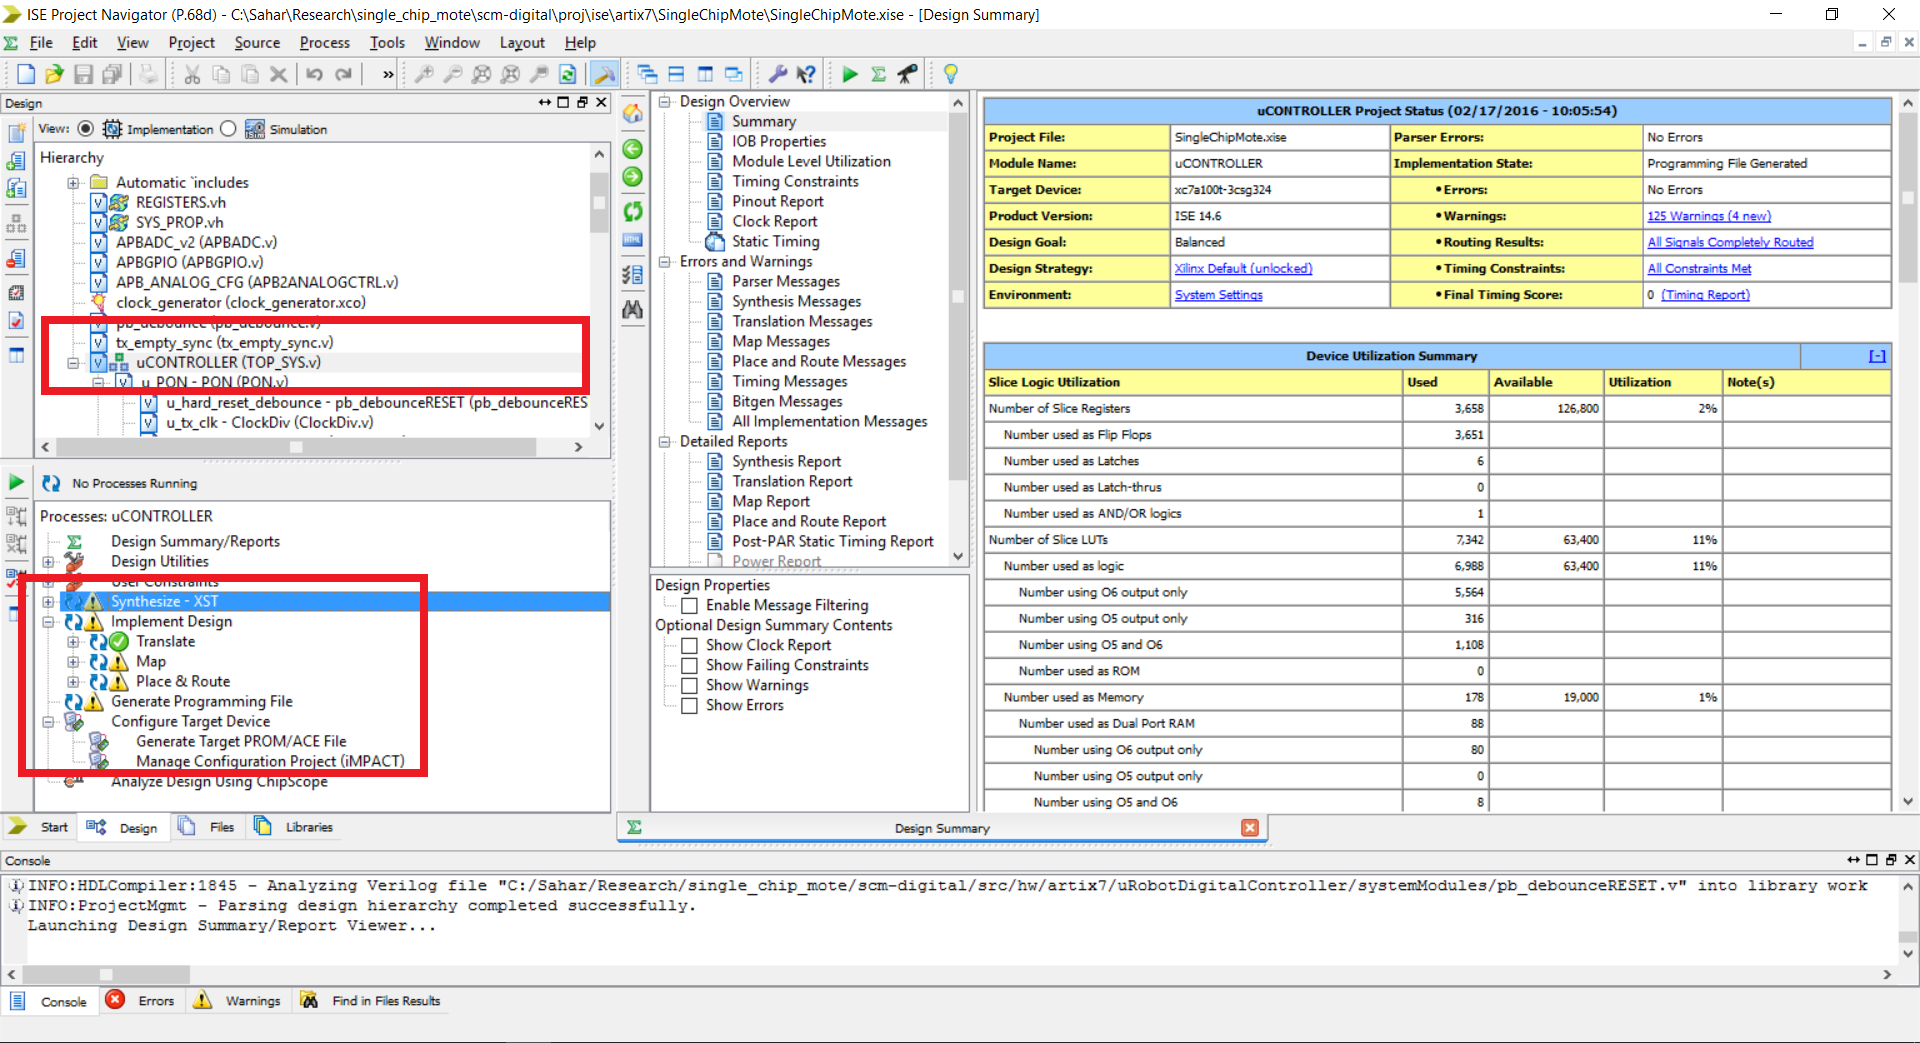
\includegraphics[width=1\linewidth]{ise-synthesis}
\caption{ISE Project Navigator for the SingleChipMote project}
\label{fig:ise-synthesis}
\end{figure}

\begin{figure}
\centering
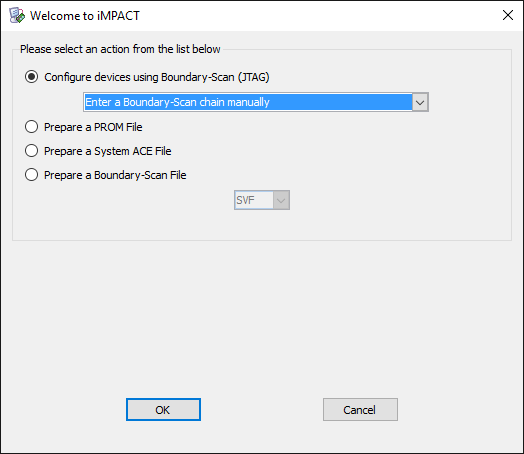
\includegraphics[width=0.7\linewidth]{impact0}
\caption{Configuring a new iMPACT Project}
\label{fig:impact0}
\end{figure}
\begin{figure}
\centering
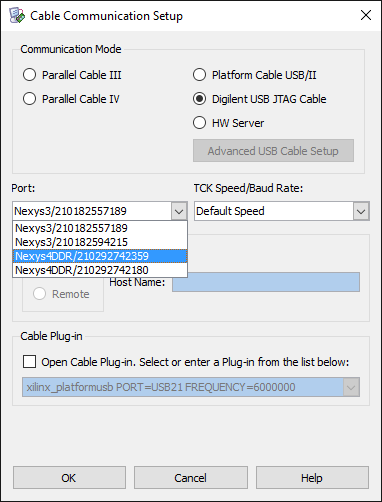
\includegraphics[width=0.7\linewidth]{impact3}
\caption{Selecting the device to program in iMPACT}
\label{fig:impact3}
\end{figure}
\begin{figure}
\centering
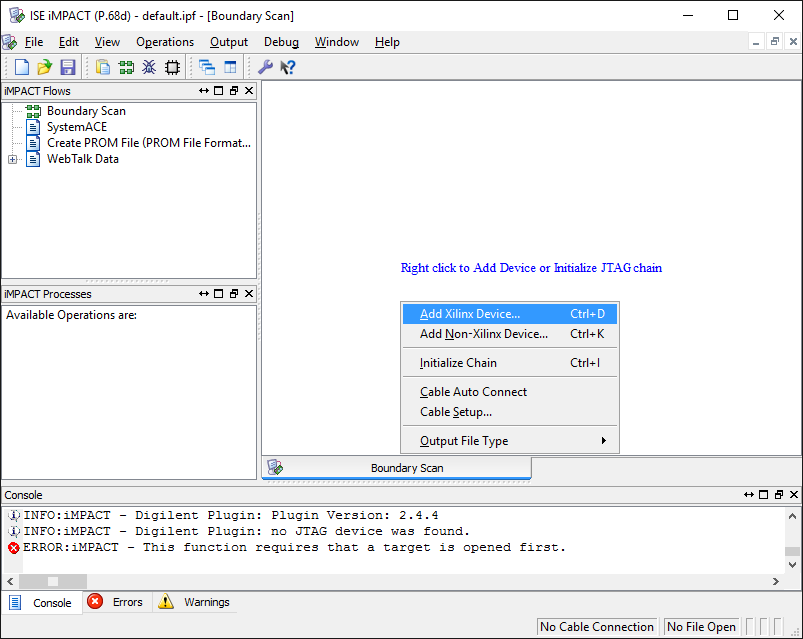
\includegraphics[width=0.7\linewidth]{impact1}
\caption{Adding a Xilinx device in iMPACT}
\label{fig:impact1}
\end{figure}
\begin{figure}
\centering
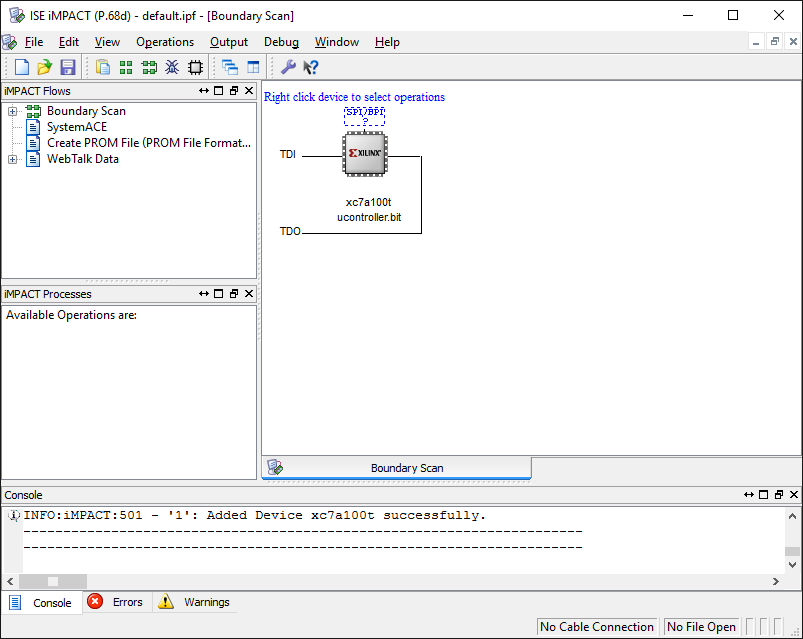
\includegraphics[width=0.7\linewidth]{impact2}
\caption{Main iMPACT window with a selected device to program}
\label{fig:impact2}
\end{figure}
\begin{figure}
\centering
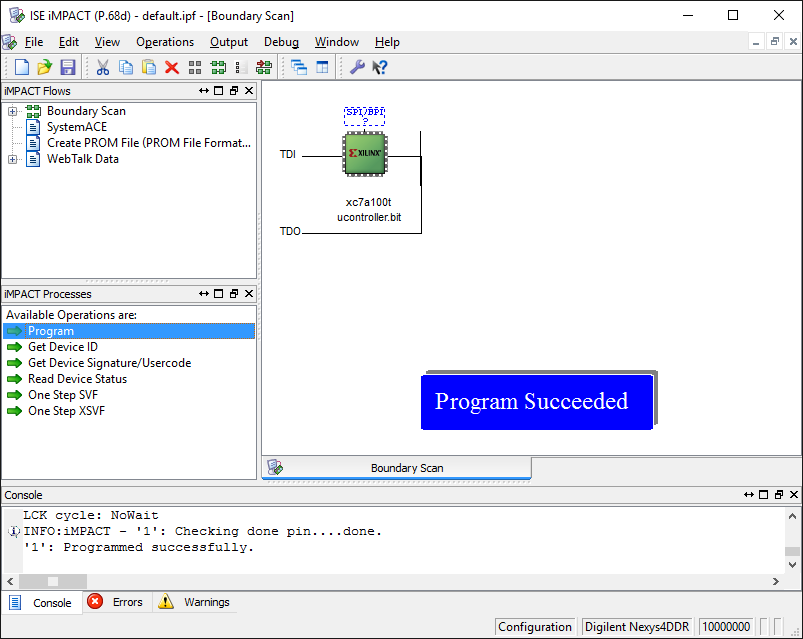
\includegraphics[width=0.7\linewidth]{impact4}
\caption{Main iMPACT window after successfully programming a device}
\label{fig:impact4}
\end{figure}

\subsection{Digilent Adept} \label{digilent-adept}
Digilent Adept is a utility provided by Digilent that can be used to load bitstream files onto some of their FPGA boards. The version of Digilent Adepet used for this project is 2.15.3; however, the latest version \cite{adept-download}, 2.16.1, is also compatible. Adept is used to program the Nexys 3 board but does not support the Nexys 4 DDR. The Nexys 3 also has additional memory external to the FPGA, written through Adept and accessed on the FPGA. This memory is used for bootloading (see chapter \ref{bootloading} for more information on bootloading), and must be written {\it before} the bitstream is loaded. \\

\textbf{Using Adept to load a bitstream file (Nexys 3 only)}

\begin{enumerate}
	\item Ensure that the power switch on the Nexys 3 board is in the ON position.
	\item Connect the Nexys 3 board to the computer using the micro-USB port on the board labled USB PROG. There is a separate micro-USB port on the board for UART communication which cannot be used for loading a bitstream. 
	\item Once the board has been recognized by the computer and the proper drivers has been installed, launch Adept.
	\item On the upper-right of the window, there is a drop-down menu listing all of the Digilent devices connected to the computer. Select the Nexys3.
	\item Go to the Config tab, select the Browse... button, and select the bitstream file generated for a Spartan-6 FPGA (for an example project on the Spartan-6, go to \path{scm-digital/proj/ise/spartan6/uRobotDigitalController/ucontroller.bit}).
	\item Press the Program button to program the FPGA (see Figure \ref{fig:adept0}).
\end{enumerate}

\textbf{Using Adept to load a file into external RAM} \\

NOTE: The memory must be written {\it before} the bitstream is loaded.
\begin{enumerate}
	\item Ensure that the power switch on the Nexys 3 board is in the ON position.
	\item Connect the Nexys 3 board to the computer using the micro-USB port on the board labled USB PROG. There is a separate micro-USB port on the board for UART communication which cannot be used for loading a bitstream. 
	\item Once the board has been recognized by the computer and the proper drivers has been installed, launch Adept.
	\item On the upper-right of the window, there is a drop-down menu listing all of the Digilent devices connected to the computer. Select the Nexys3.
	\item Go to the Memory tab. There are options to program SPI Flash, BPI Flash, and RAM. The Nexys 3 designs used for the Single Chip Mote use the RAM. 			\item Select the RAM option on the right side of the Memory tab. Then select the Browse... button in the Write File to Memory section and select the file to be written. Check the Verify check box.
	\item Select the Write button (see Figure \ref{fig:adept1}).
\end{enumerate}

For more information on how Digilent Adept is used for bootloading onto the Single Chip Mote, see section \ref{loading-sw} on connecting and loading software.

\begin{figure}
\centering
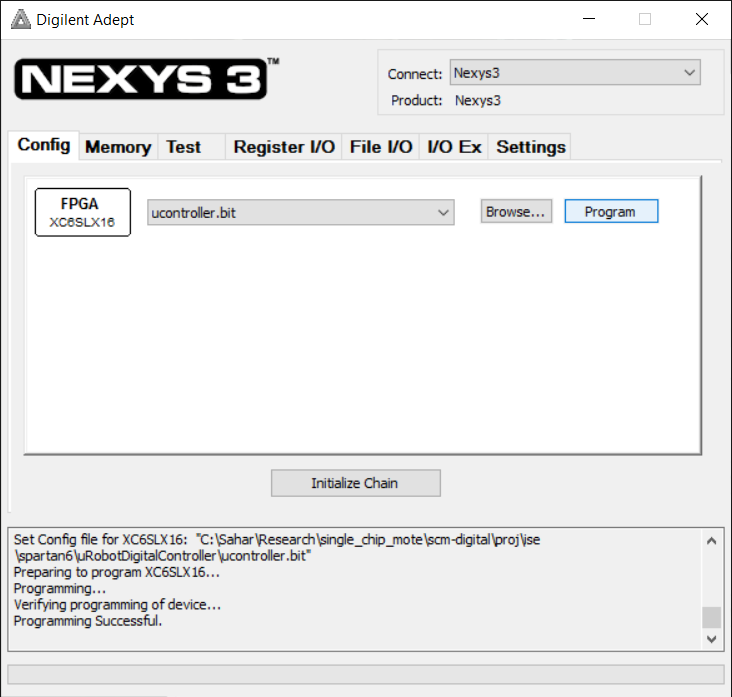
\includegraphics[width=0.7\linewidth]{adept0}
\caption{Adept settings for programming a bitstream}
\label{fig:adept0}
\end{figure}

\begin{figure}
\centering
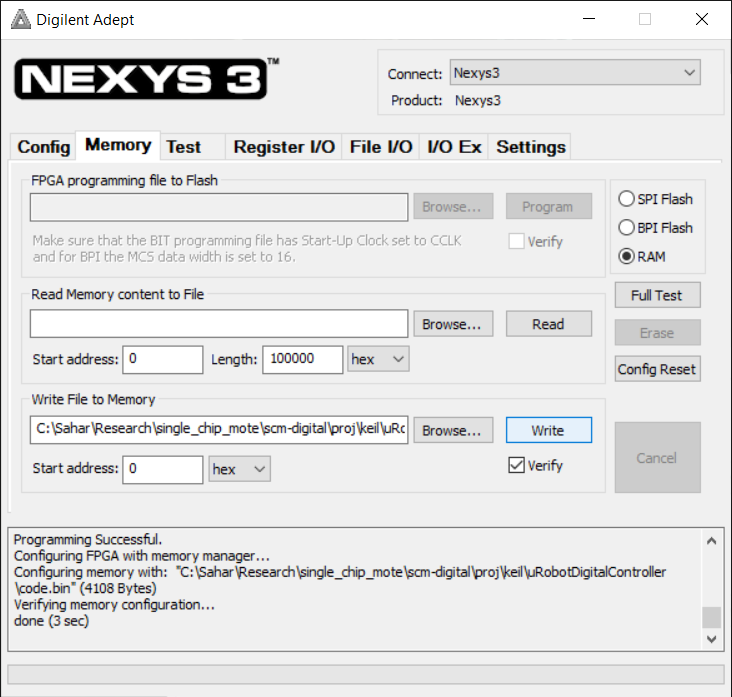
\includegraphics[width=0.7\linewidth]{adept1}
\caption{Adept settings for writing memory on the Nexys 3 board}
\label{fig:adept1}
\end{figure}

\subsection{Xilinx Vivado Design Suite}
As mentioned previously, the Vivado Design Suite can be used for designs on the Artix-7 FPGA. Xilinx and Digilent are providing increasing support for Vivado and decreasing support for ISE. However, importing the Single Chip Mote project from ISE to Vivado has not been tested, nor has it been confirmed that the UC Berkeley Xilinx license will work on earlier versions of Vivado (it will not work on anything released after October 2015). Xilinx does offer a free WEBPACK license which also has not been used or tested for the Single Chip Mote project.

\section{Software Development Tools}

\subsection{Keil uVision5} \label{keil}
Keil uVision5 is an IDE used for developing software running on ARM microprocessors. This IDE is part of the ARM MDK 5 Microcontroller Development Kit \cite{keil-download}. The version of the MDK used for this project is 5.11; however, the latest version, 5.18, is also compatible.

To compile code for the ARM Cortex M0 on the Single Chip Mote, open an existing project in Keil uVision5. The project file used for this demonstration is \path{scm-digital/proj/keil/uRobotDigitalController/code.uvprojx}. Then go to the Project menu and select Build Target. This compiles the code, creates a C binary image called code.bin, and also creates a text file called disasm.txt, containing a disassembled version of the code. The C binary image is loaded into the instruction memory of the Single Chip Mote on an FPGA using the bootloader (see chapter \ref{bootloading} for more information on bootloading).

For more information on how to make a Keil uVision5 project for the Single Chip Mote, see section \ref{keil-project-settings} on Keil project settings.

\subsection{Bin2coe} \label{bin2coe}
Bin2coe \cite{bin2coe-download} is a small Windows executable used to convert C binary image files (bin) to COE files used by Xilinx to initialize FPGA memories. COE files are used to initialize the instruction ROM with software written and compiled in Keil. This is used for the bootloading ROM on the Single Chip Mote. This program limits the data widths of the COE file to 32 bits, and therefore the generated COE files are limited to memories with a width of 32 bits.
